\chapter{Related Work}

% Try to say the "easy" or "obvious" things first (ex: define the problem)! Then describe the "standard" approach to QA and its variants.

% Define firstly the task: what exactly QA means, what are the question and answer that are expected?
A question answering system allows users to ask a question in natural language and receive an exact and succinct answer in place of a list of documents that contain the answer \cite{kato2004hia, hirschman2002nlq}. Since the first article that addressed a textual question answering system by computer was presented by Simmons (1965)\cite{simmons1965aeq}, many systems have been developed and some of the approaches have been widely used in a number of applications, for instance Okapi BM2 \cite{robertson1996ot} that will be mentioned later. A typical question answering system is showed in the Figure \ref{fig: Question Answering Architecture}.

\begin{figure}[htbp]
\centering
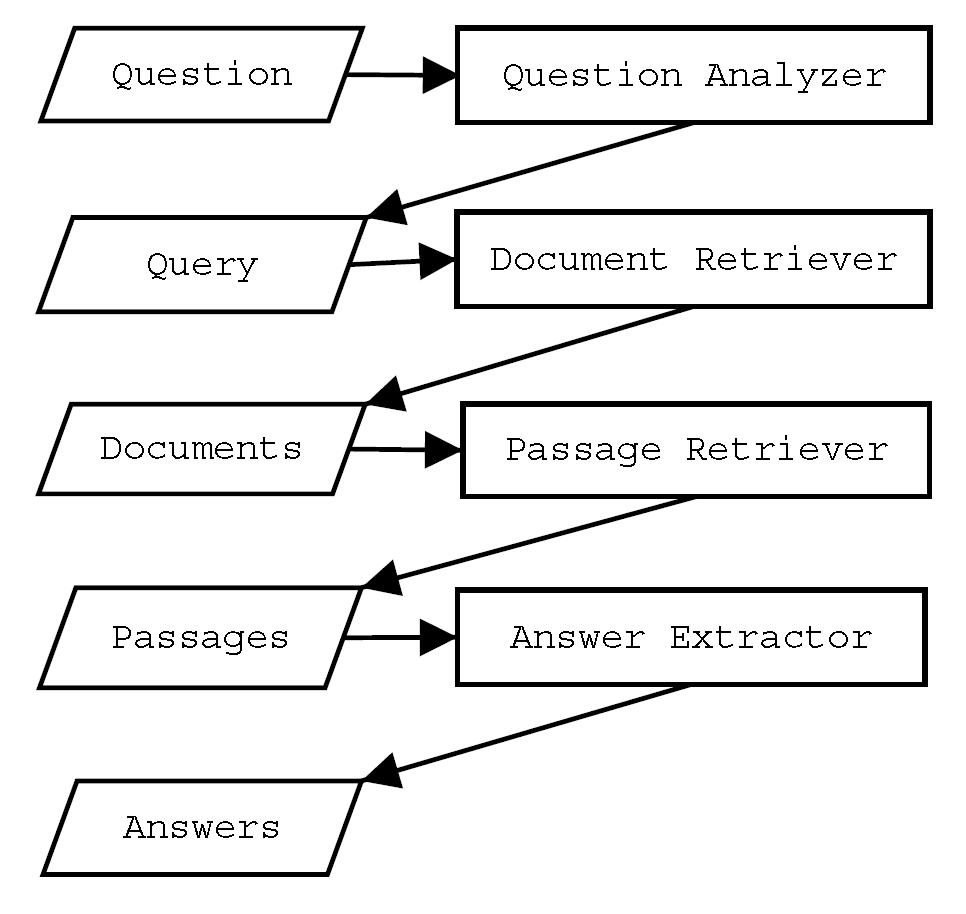
\includegraphics[scale = 0.5]{QASystem.jpg}
\caption{A typical Question Answering Architecture}
\label{fig: Question Answering Architecture}
\end{figure}

In a general question answering system, there are four major components \cite{tellex2003pmf, hirschman2002nlq,tellex2003qep, bilotti2004wbq}:

\begin{itemize}
\item {Question analysis: There are two tasks in this component. First, questions in natural language asked by a user need to be converted into queries that are needed by the subsequent parts of the system. The queries created from user's question contain terms likely to appear in documents containning an answer, for instance for such question as \textit{What is the capital of Vietnam?}, the corresponding query is \textit{capital + vietnam}. Second, the expected answer type for this question is detected in this stage so that it helps to narrow the space of searched answers. For example, questions with \textit{When} always relate to \textit{time}, thus those terms concerning time are expected such as \textit{date}, \textit{hour}, etc. }.
\item {Document retrieval: This task is to retrieve documents from the corpus that may be taken from Internet by a search engine or archived documents likely to contain answers to the query.}
\item {Passage retrieval: A passage can be simply defined as a sequence of words regardless of individual sentences or paragraphs. Some text-based information retrieval systems define a passage as a fixed-length block of words. \cite{goharian2008dsp}. Passage retrieval algorithms take a document and a question and try to return a list of passages from the document that are most likely to contain the answer information. For this,  all passages are compared with each other using passage scoring. In text-based question answering system, the score of a passage is based on the score of its words with respect to question words. The score of a question word found in a passage is calculated based on the definition of this word and/or relations of this word with other words in the text \cite{tellex2003qep}.}
\item {Answer extraction: Based on the question analysis and retrieved passages, the system extracts phrase/phrases representing an answer.}
\end{itemize}

We are only interested in the passage retrieval stage and not in the document retrieval, the question analysis nor in the answer extraction. It is because we have already had documents as meeting transcripts and the type of questions as the BET questions that are statements to be assessed. In our case, the type of answers is simply \textit{true} or \textit{false} one bit for each question. We do not need an answer as a short text extracted from the retrieved passage in which we will still have to compare two answers in order to determine the true statement. Moreover, the answer extraction is a difficult task and it can not avoid some errors. We would rather use the fully retrieved passages in determining the true statement. Thus, the stage of answer extraction is not suitable to develop in our system. For this reason, we will present only state-of-the-art methods related to passage retrieval including both traditional methods and modern methods.


Most passage retrieval algorithms calculate passage scoring based on words from the passage that are found in the question, namely matched words. However, the method of computing matched word score is different from each algorithm. 

The simplest algorithm for this approach was proposed by Light\cite{light2002aec}, in which a passage score function counts the number of words from the question found in the passage as the score for this passage. That means all words are treated equally and are given the same importance. Many question answering systems use this method as a baseline score to evaluate their performance. 

To date, there are many passage retrieval methods that have been presented in the Text Retrieval Conference (TREC) \url{http://trec.nist.gov}. These methods can be classified into two groups. One group includes traditional methods and assigns scores to each matched words independently. That means there are no relations between two matched words. Another group  considers relations amongst matched words to assign scores to them. 

For the first group, typical approaches use part-of-speech and/or frequencies of a word in order to calculate a score. Meanwhile for the second group, dependency relation among matched words in a phrase is computed to give a score for this phrase instead of words. This makes the second group more suitable to capture semantic properties than the first group.

Take SiteQ's passage retrieval algorithm \cite{lee2002seh} as an example. In this system a passage consists of some consecutive sentences segmented by punctuation and passage score is calculated by summing the weights of individual sentence in the passages. Each sentence is given a score by a formula that combines both the part-of-speech method and the query term density method. The weight of the matched words is assigned as follows: A proper noun (a common noun recognized by a capital letter) has a higher score than a verb, an adjective and/or an adverb. The term density is defined as the distance among matched words. If two sentences have the same number of matched words the sentence with smaller distance will receive a higher score.

The main idea of using word frequencies is that if a word appears many times in a current passage but only a few in other passages, its score in the current passage is higher \cite{robertson2004uid}. That means the importance of a word increases proportionally due to the number of times this word is found in a passage, but inversely to the number of times this word is found in the overall document. The simplest method for this idea is the \textit{term frequency inverse document frequency} \textit{\ensuremath{tf\times idf}}. In which, the \textit{tf} is the term frequency that measures the importance of the term \textit{\ensuremath{t_{i}}} within the document \textit{\ensuremath{d_{i}}} and \textit{idf} is the inverse document frequency that measures the importance of the term \textit{\ensuremath{t_{i}}} in the whole collection of documents. The Okapi BM25 \cite{robertson1996ot, beaulieu1995ot, xue2008rmq, comas2008sdr, tellex2003qep} presents state-of-the-art method for assigning weights to matched words using word frequencies. In fact, Okapi BM25 is a ranking function that is used to rank matching documents according to their relevance to a given query. Thus, it is often used in the Document Retrieval stage of question answering systems. However, according to the Okapi BM25 presented in the TREC-4 \cite{robertson1996ot}, this function is also used for passage determination and search. In addition, it is a complex function which was developed from the function of term frequency-inverse document frequency \textit{\ensuremath{tf\times idf}} \cite{robertson2004uid}. 

More approaches in the second group consider dependency relation among matched words, in which n-gram matching is the simplest case. The n-gram method pays more attention to the order of matching words. Accordingly, those in order are better. More specifically, this method is used to estimate similarity between two strings by examining all n-word substring matchings instead of word matchings \cite{robertson1998ang}. Another simple method is to use word density presented in the SiteQ's algorithm above. A more complex method for these approaches presented by Cui \cite{cui2005qap} uses a dependency tree to assign scores to sentences. Given the reason that one sentence in English can be written in different ways by exchanging position of words in the sentence without changing its meaning. For instance, with the sentence \textit{John wrote a science fiction book}, it may be written in some different ways but the meaning will remain unchanged. The different ways of writing the sentence include: 1)  \textit{A science fiction book was written by John}; 2) \textit{John wrote a book of science fiction}; 3) \textit{A book of science fiction was written by John}; and 4) \textit{John wrote a science fiction book}. These sentences can build a dependency tree that represents correctly positioned word relations in the sentences, so that a given query will be compared with this tree instead of one initial sentence.
 
In order to enhance the performance of question answering systems, lexical extensions for queries are added such as stemming, lemma, synonyms \cite{light2002aec}, \cite{tellex2003pmf},\cite{bilotti2004wbq}, \cite{lee2002seh}.
